\section{Reibeplätzchen}
\textit{Savory small potato-based pancakes. Can be served as a main course or dessert. Usually served with applesauce.}


\subsection*{Ingredients}
\textit{serves 2-3 as a main course, sufficient for 18-20  Reibeplätzchen}

\begin{tabular}{ l l }
  1kg & potatoes \\
  1 & egg \\
  1 & medium-sized onion \\
  1 Tbsp & oatmeal \\
  1 - 1.5 tsp & salt \\
    & oil for pan-frying (sunflower oil) \\
  % \multicolumn{2}{l}{oil for pan-frying (sunflower oil)} \\
\end{tabular}

\subsection*{Description}
\begin{enumerate}
	\item peel and grate the raw potatoes (using a kitchen grater similar to the one shown in picture 1)
	\item place the potatoes in a strainer and leave for 5-10 minutes (picture 2, 3)
	\item gently puor out the water, but keep the layer of starch at the bottom of the bowl
	\item put the potatoes, finely chopped onion, oatmeal, egg, and salt into the bowl and mix (picture 4)
	\item heat up a skillet (or two) and add some oil
	\item put one tablespoon of the mix into the skillet, spread out to create a round shapes with a thickness of 3-6 mm and a diameter of 6-10 cm (picture 5)
	\item fry for 2-3  minutes on medium to high heat, flip and fry the other side for 2-3 minutes. Add more oil when necessary (there should always be a thin layer of oil in the skillet).
	\item if not dark enough, fry a bit more from each side
	\item try the first batch and add more salt if necessary
\end{enumerate}


\begin{figure}[!htb]
    \begin{center}
    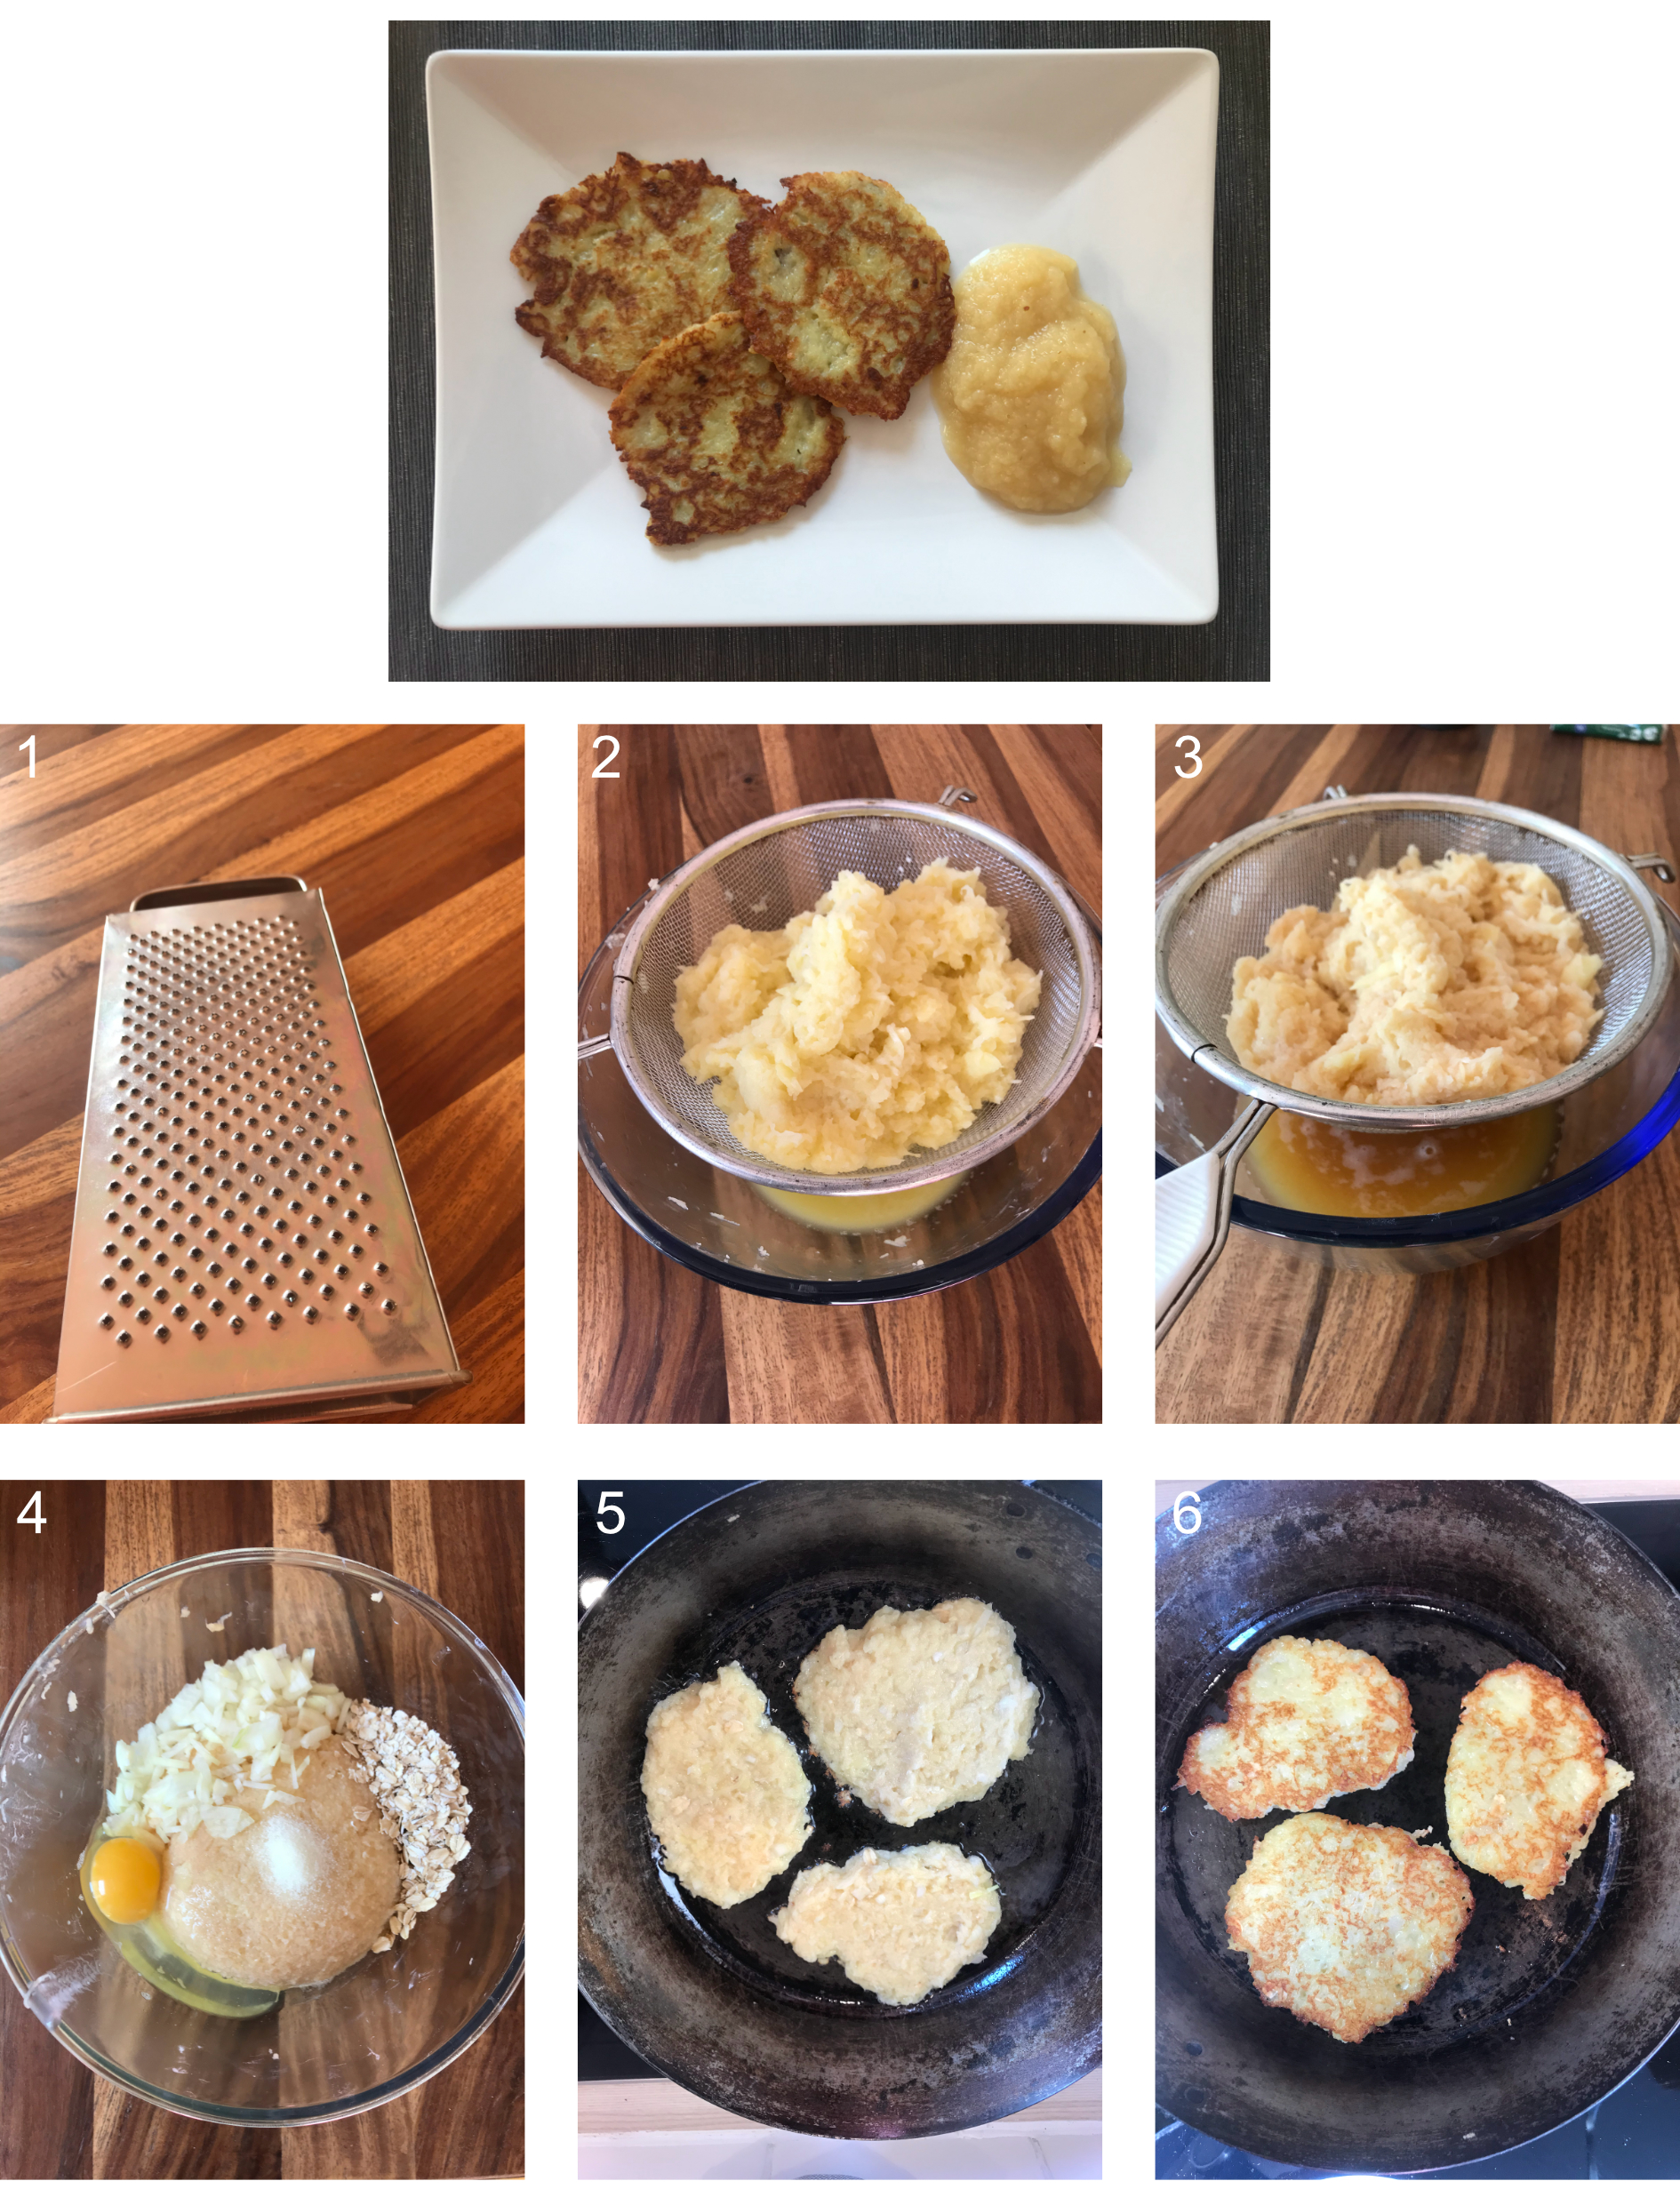
\includegraphics[width=16cm]{Pictures/Main/Reibeplaetzchen/reibeplaetzchen.jpg}
    \caption[Reibeplätzchen]{Reibeplätzchen}
    \label{fig:reibeplaetzchen}
    \end{center}
\end{figure}